%% LyX 2.0.4 created this file.  For more info, see http://www.lyx.org/.
%% Do not edit unless you really know what you are doing.
\documentclass[twocolumn,english]{IEEEtran}
\usepackage[T1]{fontenc}
\usepackage{color}
\usepackage{babel}
\usepackage{float}
\usepackage{amssymb}
\usepackage{graphicx}
\usepackage[unicode=true,
 bookmarks=true,bookmarksnumbered=true,bookmarksopen=true,bookmarksopenlevel=1,
 breaklinks=false,pdfborder={0 0 0},backref=false,colorlinks=false]
 {hyperref}
\hypersetup{pdftitle={Your Title},
 pdfauthor={Your Name},
 pdfpagelayout=OneColumn, pdfnewwindow=true, pdfstartview=XYZ, plainpages=false}

\makeatletter

%%%%%%%%%%%%%%%%%%%%%%%%%%%%%% LyX specific LaTeX commands.
%% Because html converters don't know tabularnewline
\providecommand{\tabularnewline}{\\}
\floatstyle{ruled}
\newfloat{algorithm}{tbp}{loa}
\providecommand{\algorithmname}{Algorithm}
\floatname{algorithm}{\protect\algorithmname}

%%%%%%%%%%%%%%%%%%%%%%%%%%%%%% Textclass specific LaTeX commands.
\floatstyle{ruled}
\newfloat{algorithm}{tbp}{loa}
\floatname{algorithm}{Algorithm}
\usepackage[noend]{algorithmic}
\newcommand{\forbody}[1]{ #1 \ENDFOR}
\newcommand{\ifbody}[1]{ #1  \ENDIF}
\newcommand{\whilebody}[1]{ #1  \ENDWHILE}
\renewcommand{\algorithmicprint}{\textbf{draw}}

%%%%%%%%%%%%%%%%%%%%%%%%%%%%%% User specified LaTeX commands.
% for subfigures/subtables
\ifCLASSOPTIONcompsoc
\usepackage[caption=false,font=normalsize,labelfont=sf,textfont=sf]{subfig}
\else
\usepackage[caption=false,font=footnotesize]{subfig}
\fi

\makeatother

\begin{document}

\title{Symbolic Regression with Genetic Programming}


\author{Matthew J. Urffer}


\IEEEaftertitletext{CS 528 Machine Learning, Fall 2012}
\maketitle
\begin{abstract}
Symbolic regression is a applied to an artibary function utilzing
genetic programing techniques where the genetic program is represented
by an expression tree. The initial population was generated with ramped
half and half with randomly constructed trees. Canidates for the next
generation were chosen by tournament selection and rank selection
based on the fitness of the individual where the fitness was determined
by the sum square error (SSE). These individuals were subject to crossover
and heavily mutated. It was determined that the best fitness an individual
could achieve was an SSE around 9.3, which is much higher than the
goal of 0.5.\end{abstract}
\begin{IEEEkeywords}
symbolic regression, genetic programming, expression trees
\end{IEEEkeywords}

\section{Introduction}

\IEEEPARstart{ R}{egression} is utilized heavily in all fields
when the the functional form is known and only the coefficients have
to be determined. When the functional form is not known a functional
form has to be infered from the underlying model which can often be
difficult to derive and fraught with assumptions. Symbolic regression
(function discovery on a multivariate daa set) is a form of regression
in which the functional form and the coefficients are determeind.
Symoblic regression is then very differnet but similar to regular
regression; in regression the functional form is known and only the
coefficients need to be determined while in symbolic regression the
coefficients and the functional form are not known. In regression
it is possible to follow the gradient of the error surface for rapid
convergence, but for symbolic no such error surface exists, and therefore
a different type of search is required. Genetic programming is an
automated method for creating solutions to high level statement of
the problem by evolving individual solutions in order to optimize
a fitness function is then an ideal method to solve this problem.
Genetic programming attemps to mimic the evolutionary process by creating
an intial population, only letting the best individuals in a population
reproduce, and using an anolgy of DNA mutations and the crossing of
genetic material that occurs during breeding.


\section{Methodology}

A symbolic regression individual was modeled using an a recursively
defined expression tree. An initial population (forest) of trees was
generated and the fitness was computed for each of the individuals.
Generations of the forest were computed utilizing genetic operators
to evolve the old generation into the new. The following sections
explain each part in detail.


\subsection{Expression Tree Representation}

Expression trees were used to represent symbolic functional forms
due to their ease of use and the ability to easily apply genetic operators
such as crossover and mutations. The expression trees were implemented
recursively in c as linked nodes. Trees where created recursively
in a doubly linked list. Provided a maximim depth, the function would
call itself until the the maximum depth was reached. The option to
prune the trees to create a more diverse intitial tree structure was
also implemented, but in practice preliminary pruning made an insignificant
differnece on the final results and was not used. The algorthim is
shown in Algorthim \ref{TreeCreation}. All of the operators were
represented as strings, with the evaluation of a tree preformed by
a series of case statements. The unary functions cos and sin where
overloaded to contain an additional competent which represents the
magnitude. Trees were constructed in a random manner, with equal probability
of picking any operator from the function set. A terminal node was
chosen either by max depth or a pruning probability. Terminal node
operators (values) where not chosen with a user supplied probability.
In addition the terminal set only included two operators, \texttt{x}
and \texttt{value}. The \texttt{x} operator represented the value
on which to evaluate the expression tree, while the \texttt{value
}keyword represented a real number uniformly chosen on the interval
(-1,1). Table \ref{FunTermSet} enumerates the function and terminals
sets used.

\begin{table}[htbp]
\caption{Function and Terminal Set}


\begin{tabular}{|c|c|}
\hline 
 & Operators\tabularnewline
\hline 
\hline 
Function Set & $b\sin a,\newline b\cos a,\newline b\sqrt{\left|a\right|},\newline\left|a\right|^{b},\newline+,\newline-,\newline\times,\newline+$\tabularnewline
\hline 
Terminal Set & $x\newline,\mathbb{R}$\tabularnewline
\hline 
\end{tabular}\label{FunTermSet}
\end{table}


\begin{algorithm}[tbh]
\texttt{node {*}buildTree(node{*} parent,int depth, double pruneProb,
double constProb)\{}

\texttt{\,node {*}tree = NULL;}

\texttt{\,if (depth == 0 || (drand(0,1) < pruneProb \&\& parent !=
NULL)) \{}

\texttt{\,\,tree = leafNode(constProb); }

\texttt{\,\,tree->parent = parent;}

\texttt{\,\,return tree;}

\texttt{\,\}else\{}

\texttt{\,\,node {*}tree = funcNode();}

\texttt{\,\,tree->parent = parent;}

\texttt{\,\,tree->left = buildTree(tree,depth-1,}

\texttt{pruneProb,constProb);}

\texttt{\,\,tree->right= buildTree(tree,depth-1,}

\texttt{pruneProb,constProb);}

\texttt{\,\,return tree;}

\texttt{\,\}}

\texttt{\} }

\caption{Random Tree Creation}


\label{TreeCreation}
\end{algorithm}



\subsection{Initial Population}

The initial population was generated using ramped half and half in
which half of the population are randomly generated trees to the maximum
depth, while the other half of the population was created of full
trees ranging from a tree depth of 2 to the maximum depth. The initial
population was assured to have no duplicates (by comparing tree structure).
It is possible that trees with different structures evaluate to the
same result, an example of which is provided in Figure \ref{SimilarTree}.

\textbf{}
\begin{figure}[tbh]
\includegraphics[width=3in]{GeneticProgrammingExpressionTreeFigures_SameTreeNotEqual}

\label{SimilarTree}

\textbf{\caption{Semantically different trees can mathematically be equivalent}
}

\end{figure}



\subsection{Genetic Algorithm}

The genetic algorithm typically consist of four tasks: creating an
initial population, evaluating that populations fitness, selecting
members of the current population to breed, and then applying genetic
operators to the selected members to breed the new population. This
is completed for either a maximum generation is reached or the desired
fitness is achieved. In the symbolic regression problem the fitness
of an individual is defined as the sum squared error with lower fitness
being considered desirable.

\begin{algorithm}[tbh]
\begin{algorithmic}
[1]\WHILE{$error>goal$}

\whilebody{\FORALL{$t\in F$}

\forbody{\STATE{Compute fitness}}

\FORALL{$t\in F$}

\forbody{\STATE{Choose individuals based on fitness}

\STATE{Select individuals for next population}

\STATE{Crossover selected individuals}

\STATE{Mutate selected individual}}}
\end{algorithmic}


\caption{Genetic Program Outline}


\label{AlgoOutline}
\end{algorithm}



\subsection{Population Selection}

Population selection was achieved using a hybrid approach of tournament
selection and rank selection. In rank selection the individuals were
selected based on their rank, where the rank was determined by their
fitness (lower SSE correspond to a higher fitness). Tournament selection
was used to generate the other component of the population for breeding.
Two trees were chosen at random from the entire population and the
tree with the highest fitness was added to the population for breeding.
There was no restriction on trees being selected more than once. Algorithm
\ref{PopSelectionAlgo} outlines this approach.

\begin{algorithm}[tbh]
\begin{algorithmic}
[1]\WHILE{$numAdded<population$Size}

\whilebody{\STATE{Determine tournament selection fraction}

\STATE{Determine rank selection fraction}

\STATE{Rank population members based on fitness}

Preform Rank Selection

\WHILE{i < TotalRankNumber}

\whilebody{\STATE{Copy ranked tree i}}

\WHILE{j < TotalTournamentNumber}

\whilebody{\PRINT{a random tree, t1}

\PRINT{a random tree, t2}

\IF{fitness(t1) > fitness(t2)}

\STATE{keep t1}

\ELSIF{fitness(t1) < fitness(t2)}

\STATE{keep t2}

\ENDIF{}}}
\end{algorithmic}


\caption{Canidate selection for the next population}


\label{PopSelectionAlgo}
\end{algorithm}



\subsection{Genetic Operators}

Individuals selected for reproduction are subjected to genetic operators
to breed the next generation. Genetic programs generally contain two
genetic operators, crossover and mutation. Crossover serves to create
new members of the population by interchanging the genetic material
(tree structure) of two parents in which significant changes in the
tree solutions are achieved. Mutation serves to slightly modify an
existing solution. 


\subsubsection{Crossover}

Crossover is defined in genetic programming as the swapping of sub-trees
between individuals in the population, which is meant to mimic the
crossover of genes that occurs during evolution. As the solutions
are recursively defined, crossover was implemented by selecting randomly
selecting a two nodes from different trees and swapping their parents.

\begin{figure}[tbh]
\includegraphics[width=3in]{GeneticProgrammingExpressionTreeFigures_CrossOver}

\caption{Example of Crossover}


\label{CrossOver}
\end{figure}



\subsubsection{Mutation}

Mutation, unlike crossover, does not involve changes to the structure
of the solution but rather operators within the solution. For example,
in symbolic regression mutation will randomly (defined by the mutation
rate) change the node function and leaf values, but it will not add
or prune branches to the tree structure. Mutation was implemented
as a recursive traversal of the tree, switching the function types
with other functions types according to a user supplied probability.
The terminals mutations were implemented in a similar fashion, but
if the node was a value leaf the leaf was randomly set to a new random
variable. An example of mutation is shown in Figure \ref{Mutation}.

\begin{figure}[htbp]
\includegraphics[width=3in]{GeneticProgrammingExpressionTreeFigures_Mutation}

\label{Mutation}

\caption{Example of mutation}
\end{figure}



\section{Results}

Preliminary trials were completed at various depths in order to determine
the optimal tree depth for the problem. Population sizes were set
to be 500 individuals, and the genetic operators were completed for
50 generations. The initial populations were generated using a ramped
half and half method. Tree depths were chosen to be 6, 8, 10, 12 and
14. As shown in Figure \ref{treeDepthStudy} smaller tree sizes tended
to preform better than larger tree sizes. It was then determined that
the best tree size would be around a tree depth of 8.

\begin{figure}[tbh]
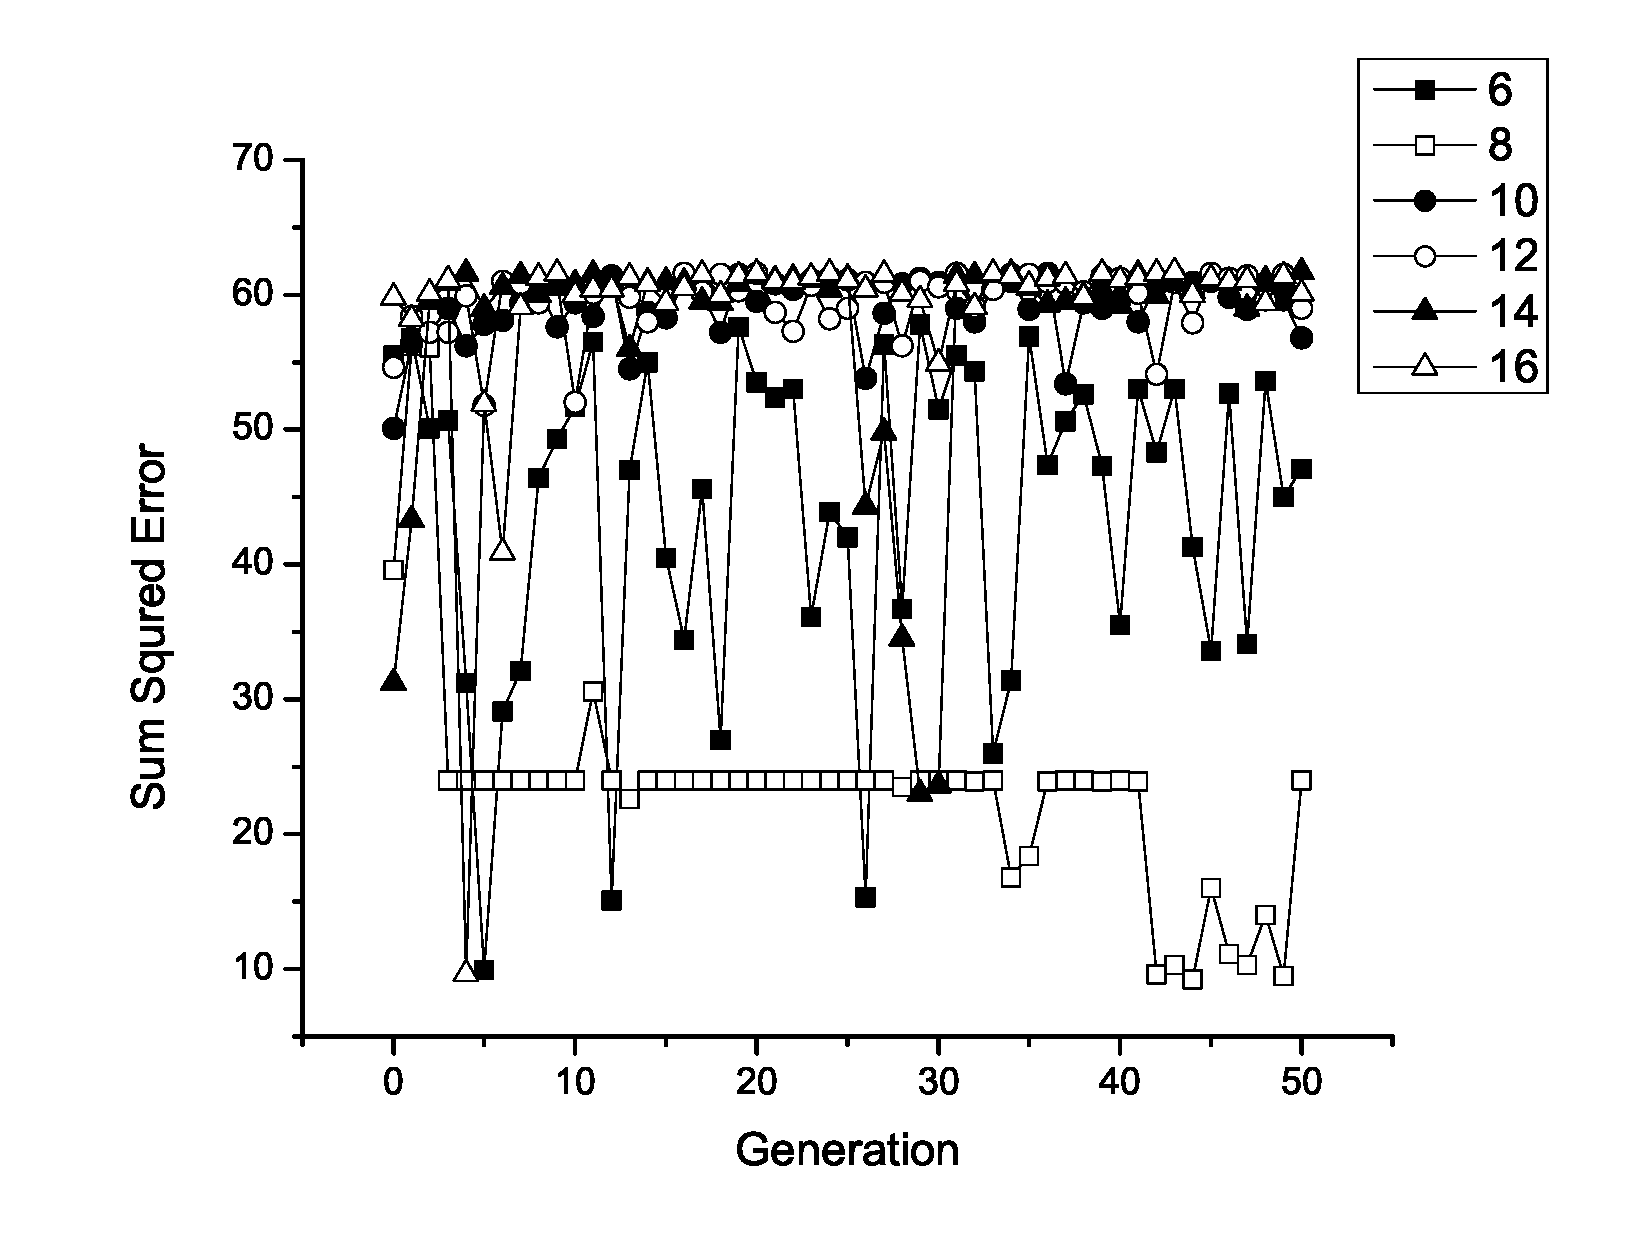
\includegraphics[width=3.5in]{Graph1}

\caption{Sum Squared Error per Generation for various tree depths. Populations
were maitained at 500 individuals, choosen with ramped half and half.}
\label{treeDepthStudy}

\end{figure}


\begin{figure}[tbh]
\includegraphics[width=3.5in]{Graph4}

\caption{Diversity of the population (1,000 trees of Depth 6)}
\label{DiversityBest}
\end{figure}


It was discovered that for a large population size (1,000) individuals
the diversity only minorly changed from the population being fully
diverse. This is to be expected in this implementation of the problem
because the value nodes are compared by the node value and it is unlikely
for two randomly drawn real values be equal (Figure \ref{DiversityBest}).
None of the trees generated had an sum squared error in the target
range of 0.5. The best expression tree generated had a sum squared
error of 9.30 with the functional form of (1), while the expression
tree is shown in Figure \ref{BestExprTree}.

\begin{equation}
a\cos x
\end{equation}
\label{bestTreeEqn}

Various attempts were made to attempt to avoid this local minima but
none proved successful. The first attempt was to introduce an very
large mutation rate (90\%), but without restricting a periodic function
from occurring near the root of the tree this only resulted in another
tree being switched to a periodic function and taking the previous
spartan's place. It was then attempted to introduce large crossover,
but if the cosine was the root node in the tree (as it is for a SSE
of \textasciitilde{}10) this only served to modify the inputs to the
cosine, to which the cosine is generally resilient. The final attempt
was to increase the minimum depth in the ramped half and half, but
this resulted in trees that had SSE's in the 100 after a few hundred
generations and was discarded.

\begin{figure}[htbp]
\begin{centering}
\textsf{\includegraphics{bestTree}\label{BestExprTree}}
\par\end{centering}

\caption{Expression Tree of optimal solution}
\end{figure}


\begin{figure}[tbh]
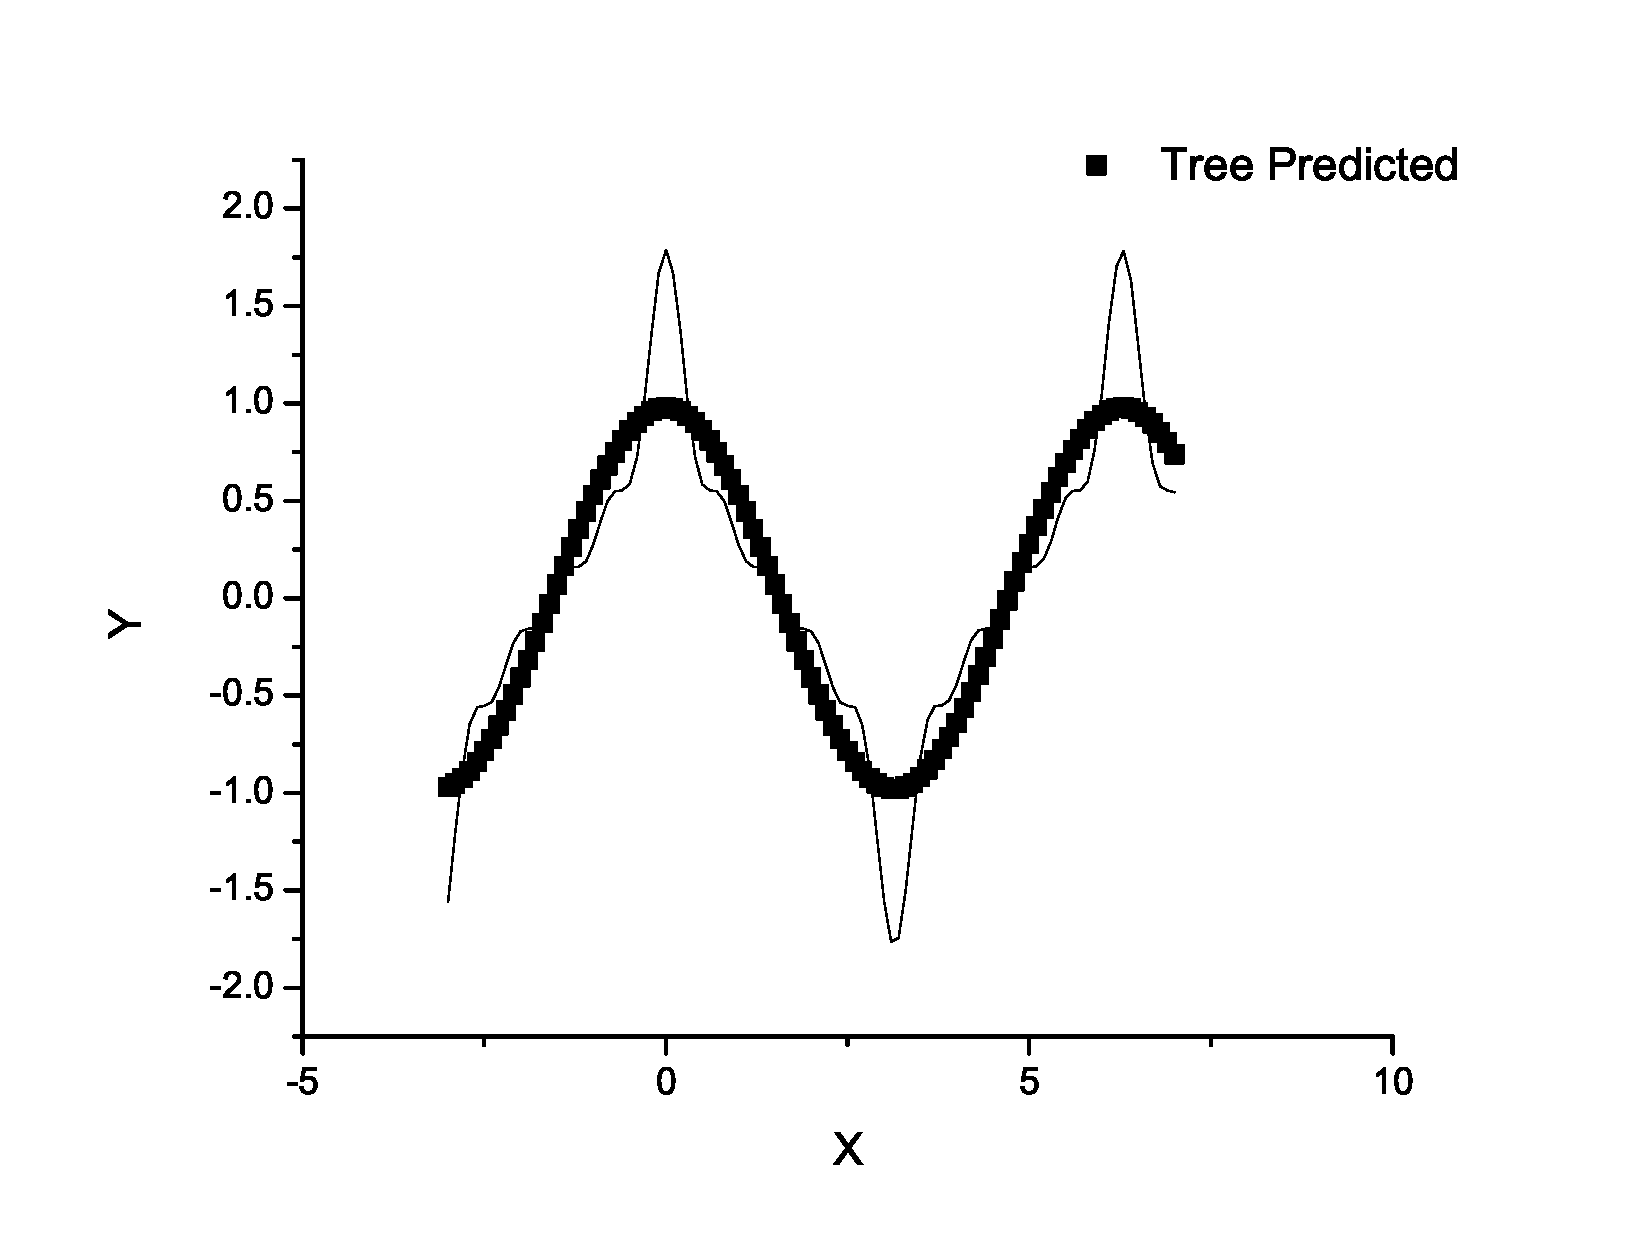
\includegraphics[width=3.5in]{Graph5}

\caption{Comparison between data and generated model}
\label{FitComparison}

\end{figure}



\section{Conclusions}

Genetic algorithms have been demonstrated to have the capability of
performing simple symbolic regression. It is well known that genetic
algorithms can preform complex symbolic regression, but as implemented
the algorithm was only capable of building a model that captured the
first order behavior of the model (Figure \ref{FitComparison}). It
is thought that unless a way is devised to avoid the local minima
provided by the cosine a genetic solution to this problem will have
a difficult time converging in a timely manner. This can be cast in
evolutionary terms where some mutations might make an individual more
fit (such as pigs having wings), but because the species is already
pretty well suited the mutation is not very likely. Future work could
be directed into casting the problem into a light such that solutions
are heavily penalized for being in this local minima. Such a method
might be to transform the data into a space (perhaps with a Fourier
transform) where only the optimal solution is favored.


\section*{Acknowledgment}

The assistantship of Matthew Lish is gratefully acknowledged with
the suggestion to overload the unary functions. Mike Franklin also
provided valuable insights on program convergence, but sadly they
didn't seem to help in this implementation.
\end{document}
